\tikzstyle{undir} = [thick]
\tikzstyle{dir} = [thick, ->, bend left = 10]
\tikzstyle{ver} = [thick, ->, draw, circle]

\begin{tikzpicture}[black, >=latex]
    \node[ver] (A) at (0, 0) {};
    \node[ver] (B) at (1.9, 1.9) {};
    \node[ver] (C) at (3, 0) {};
    \node[ver] (D) at (4, 1.2) {};
    \node[ver] (E) at (3.3, 3.7) {};
    \node[ver] (F) at (-0.5, 3) {};
    \node at (0, -0.2) {};

    \only<1>{
        \draw[undir] (A) to (B);
        \draw[undir] (A) to (C);
        \draw[undir] (B) to (C);
        \draw[undir] (C) to (D);
        \draw[undir] (B) to (D);
        \draw[undir] (D) to (E);
        \draw[undir] (E) to (F);
        \draw[undir] (F) to (A);
        \draw[undir] (B) to (F);
    }
    
	\only<2->{
        \draw[dir] (A) to (B);
        \draw[dir] (A) to (C);
        \draw[dir] (B) to (C);
        \draw[dir] (C) to (D);
        \draw[dir] (B) to (D);
        \draw[dir] (D) to (E);
        \draw[dir] (E) to (F);
        \draw[dir] (F) to (A);
        \draw[dir] (B) to (F);

        \draw[dir] (B) to (A);
        \draw[dir] (C) to (A);
        \draw[dir] (C) to (B);
        \draw[dir] (D) to (C);
        \draw[dir] (D) to (B);
        \draw[dir] (E) to (D);
        \draw[dir] (F) to (E);
        \draw[dir] (A) to (F);
        \draw[dir] (F) to (B);
    }
\end{tikzpicture}
